% Options for packages loaded elsewhere
\PassOptionsToPackage{unicode}{hyperref}
\PassOptionsToPackage{hyphens}{url}
%
\documentclass[
  9pt,
  ignorenonframetext,
  aspectratio=169,
]{beamer}
\usepackage{pgfpages}
\setbeamertemplate{caption}[numbered]
\setbeamertemplate{caption label separator}{: }
\setbeamercolor{caption name}{fg=normal text.fg}
\beamertemplatenavigationsymbolsempty
% Prevent slide breaks in the middle of a paragraph
\widowpenalties 1 10000
\raggedbottom

\usepackage{amsmath,amssymb}
\usepackage{iftex}
\ifPDFTeX
  \usepackage[T1]{fontenc}
  \usepackage[utf8]{inputenc}
  \usepackage{textcomp} % provide euro and other symbols
\else % if luatex or xetex
  \usepackage{unicode-math}
  \defaultfontfeatures{Scale=MatchLowercase}
  \defaultfontfeatures[\rmfamily]{Ligatures=TeX,Scale=1}
\fi
\usepackage{lmodern}
\ifPDFTeX\else  
    % xetex/luatex font selection
\fi
% Use upquote if available, for straight quotes in verbatim environments
\IfFileExists{upquote.sty}{\usepackage{upquote}}{}
\IfFileExists{microtype.sty}{% use microtype if available
  \usepackage[]{microtype}
  \UseMicrotypeSet[protrusion]{basicmath} % disable protrusion for tt fonts
}{}
\makeatletter
\@ifundefined{KOMAClassName}{% if non-KOMA class
  \IfFileExists{parskip.sty}{%
    \usepackage{parskip}
  }{% else
    \setlength{\parindent}{0pt}
    \setlength{\parskip}{6pt plus 2pt minus 1pt}}
}{% if KOMA class
  \KOMAoptions{parskip=half}}
\makeatother
\usepackage{xcolor}
\newif\ifbibliography
\setlength{\emergencystretch}{3em} % prevent overfull lines
\setcounter{secnumdepth}{-\maxdimen} % remove section numbering

\usepackage{color}
\usepackage{fancyvrb}
\newcommand{\VerbBar}{|}
\newcommand{\VERB}{\Verb[commandchars=\\\{\}]}
\DefineVerbatimEnvironment{Highlighting}{Verbatim}{commandchars=\\\{\}}
% Add ',fontsize=\small' for more characters per line
\usepackage{framed}
\definecolor{shadecolor}{RGB}{241,243,245}
\newenvironment{Shaded}{\begin{snugshade}}{\end{snugshade}}
\newcommand{\AlertTok}[1]{\textcolor[rgb]{0.68,0.00,0.00}{#1}}
\newcommand{\AnnotationTok}[1]{\textcolor[rgb]{0.37,0.37,0.37}{#1}}
\newcommand{\AttributeTok}[1]{\textcolor[rgb]{0.40,0.45,0.13}{#1}}
\newcommand{\BaseNTok}[1]{\textcolor[rgb]{0.68,0.00,0.00}{#1}}
\newcommand{\BuiltInTok}[1]{\textcolor[rgb]{0.00,0.23,0.31}{#1}}
\newcommand{\CharTok}[1]{\textcolor[rgb]{0.13,0.47,0.30}{#1}}
\newcommand{\CommentTok}[1]{\textcolor[rgb]{0.37,0.37,0.37}{#1}}
\newcommand{\CommentVarTok}[1]{\textcolor[rgb]{0.37,0.37,0.37}{\textit{#1}}}
\newcommand{\ConstantTok}[1]{\textcolor[rgb]{0.56,0.35,0.01}{#1}}
\newcommand{\ControlFlowTok}[1]{\textcolor[rgb]{0.00,0.23,0.31}{\textbf{#1}}}
\newcommand{\DataTypeTok}[1]{\textcolor[rgb]{0.68,0.00,0.00}{#1}}
\newcommand{\DecValTok}[1]{\textcolor[rgb]{0.68,0.00,0.00}{#1}}
\newcommand{\DocumentationTok}[1]{\textcolor[rgb]{0.37,0.37,0.37}{\textit{#1}}}
\newcommand{\ErrorTok}[1]{\textcolor[rgb]{0.68,0.00,0.00}{#1}}
\newcommand{\ExtensionTok}[1]{\textcolor[rgb]{0.00,0.23,0.31}{#1}}
\newcommand{\FloatTok}[1]{\textcolor[rgb]{0.68,0.00,0.00}{#1}}
\newcommand{\FunctionTok}[1]{\textcolor[rgb]{0.28,0.35,0.67}{#1}}
\newcommand{\ImportTok}[1]{\textcolor[rgb]{0.00,0.46,0.62}{#1}}
\newcommand{\InformationTok}[1]{\textcolor[rgb]{0.37,0.37,0.37}{#1}}
\newcommand{\KeywordTok}[1]{\textcolor[rgb]{0.00,0.23,0.31}{\textbf{#1}}}
\newcommand{\NormalTok}[1]{\textcolor[rgb]{0.00,0.23,0.31}{#1}}
\newcommand{\OperatorTok}[1]{\textcolor[rgb]{0.37,0.37,0.37}{#1}}
\newcommand{\OtherTok}[1]{\textcolor[rgb]{0.00,0.23,0.31}{#1}}
\newcommand{\PreprocessorTok}[1]{\textcolor[rgb]{0.68,0.00,0.00}{#1}}
\newcommand{\RegionMarkerTok}[1]{\textcolor[rgb]{0.00,0.23,0.31}{#1}}
\newcommand{\SpecialCharTok}[1]{\textcolor[rgb]{0.37,0.37,0.37}{#1}}
\newcommand{\SpecialStringTok}[1]{\textcolor[rgb]{0.13,0.47,0.30}{#1}}
\newcommand{\StringTok}[1]{\textcolor[rgb]{0.13,0.47,0.30}{#1}}
\newcommand{\VariableTok}[1]{\textcolor[rgb]{0.07,0.07,0.07}{#1}}
\newcommand{\VerbatimStringTok}[1]{\textcolor[rgb]{0.13,0.47,0.30}{#1}}
\newcommand{\WarningTok}[1]{\textcolor[rgb]{0.37,0.37,0.37}{\textit{#1}}}

\providecommand{\tightlist}{%
  \setlength{\itemsep}{0pt}\setlength{\parskip}{0pt}}\usepackage{longtable,booktabs,array}
\usepackage{calc} % for calculating minipage widths
\usepackage{caption}
% Make caption package work with longtable
\makeatletter
\def\fnum@table{\tablename~\thetable}
\makeatother
\usepackage{graphicx}
\makeatletter
\def\maxwidth{\ifdim\Gin@nat@width>\linewidth\linewidth\else\Gin@nat@width\fi}
\def\maxheight{\ifdim\Gin@nat@height>\textheight\textheight\else\Gin@nat@height\fi}
\makeatother
% Scale images if necessary, so that they will not overflow the page
% margins by default, and it is still possible to overwrite the defaults
% using explicit options in \includegraphics[width, height, ...]{}
\setkeys{Gin}{width=\maxwidth,height=\maxheight,keepaspectratio}
% Set default figure placement to htbp
\makeatletter
\def\fps@figure{htbp}
\makeatother

\PassOptionsToPackage{backref=page}{hyperref}

%%% === ADDITIONAL PACKAGES
\usepackage{animate}
\usepackage{caption}
\usepackage{subcaption}
\usepackage{tikz}
\usepackage{cancel}
\usepackage{booktabs}
\usepackage{stmaryrd}
\usepackage[export]{adjustbox}
\usepackage{fontawesome5}
\usepackage{algorithmic}
\usepackage{amsmath}
\usepackage{yfonts}
\graphicspath{{../files/}}

% \LinesNumbered
\newcommand{\theHalgorithm}{\arabic{algorithm}}
% \newcommand{\theHtable}{\thetable}
\usepackage[ruled,vlined]{algorithm2e}
\renewcommand{\algorithmicrequire}{\textbf{Input:}}
\renewcommand{\algorithmicensure}{\textbf{Output:}}
\newcommand{\vect}[1]{\boldsymbol{\mathbf{#1}}}

%%% === CONDITIONAL PACKAGE
\usepackage{ifthen}

%%% === TEMPLATE
\setbeamerfont{title}{series=\bfseries}
\setbeamerfont{frametitle}{series=\bfseries, size=\fontsize{12}{14}}

\setbeamersize
{
    text margin left=0.214cm,
    text margin right=0.214cm
}

\usefonttheme[onlymath]{serif}
\setbeamertemplate{bibliography item}{\insertbiblabel}
\setbeamertemplate{itemize items}[circle] % For level-1 itemize
\setbeamertemplate{itemize subitem}[circle] % For level-2 (subitems)
\setbeamertemplate{itemize subsubitem}[circle] % For level-3 (subsubitems)

\addtobeamertemplate{footline}{\raisebox{-1.3pt}{\href{https://fmin.xyz}{
\includegraphics[width=1cm]{logo.pdf}}} \hspace{0.2cm} \hbox{\insertsection \hspace{0.2cm}} \hfill \href{https://hse25.fmin.xyz}{\faGem[regular]} \hspace{0.04cm} \href{https://github.com/MerkulovDaniil/hse25}{\faGithub} \hspace{0.07cm} \href{https://t.me/fminxyz}{\faTelegram} \hspace{0.4cm}\hbox{\insertframenumber \hspace{0.1cm}}
  \vskip0pt
}

\usenavigationsymbolstemplate{}

%%% === ADDITIONAL COMMANDS
\newcommand*{\Scale}[2][4]{\scalebox{#1}{$#2$}}%
\newcommand{\argmin}{\operatornamewithlimits{argmin}}
\newcommand{\argmax}{\operatornamewithlimits{argmax}}
\newcommand{\la}{\langle}
\newcommand{\ra}{\rangle}

%%% === BACKGROUND IMAGE SETUP
\AtBeginDocument{
  \ifthenelse{\isundefined{\bgimage}}{
    % No background image specified
  }{
    \setbeamertemplate{title page}{
      \begin{tikzpicture}[remember picture,overlay]
        \node[anchor=center, xshift=0pt, yshift=0pt] at (current page.center) {
          \includegraphics[width=1.05\paperwidth, height=1.05\paperheight]{\bgimage}
        };
        \node[fill=white, fill opacity=0.7, text opacity=1, inner sep=10pt, rounded corners=10pt] at (current page.center) {
          \begin{minipage}{0.5\paperwidth}
            \centering
            \usebeamerfont{title}\inserttitle\par
            \vspace*{0.5cm}
            \usebeamerfont{author}\insertauthor\par
            \vspace*{0.5cm}
            \usebeamerfont{institute}\insertinstitute\par
          \end{minipage}
        };
      \end{tikzpicture}
    }
  }
}
\makeatletter
\@ifpackageloaded{tcolorbox}{}{\usepackage[skins,breakable]{tcolorbox}}
\@ifpackageloaded{fontawesome5}{}{\usepackage{fontawesome5}}
\definecolor{quarto-callout-color}{HTML}{909090}
\definecolor{quarto-callout-note-color}{HTML}{0758E5}
\definecolor{quarto-callout-important-color}{HTML}{CC1914}
\definecolor{quarto-callout-warning-color}{HTML}{EB9113}
\definecolor{quarto-callout-tip-color}{HTML}{00A047}
\definecolor{quarto-callout-caution-color}{HTML}{FC5300}
\definecolor{quarto-callout-color-frame}{HTML}{acacac}
\definecolor{quarto-callout-note-color-frame}{HTML}{4582ec}
\definecolor{quarto-callout-important-color-frame}{HTML}{d9534f}
\definecolor{quarto-callout-warning-color-frame}{HTML}{f0ad4e}
\definecolor{quarto-callout-tip-color-frame}{HTML}{02b875}
\definecolor{quarto-callout-caution-color-frame}{HTML}{fd7e14}
\makeatother
\makeatletter
\@ifpackageloaded{caption}{}{\usepackage{caption}}
\AtBeginDocument{%
\ifdefined\contentsname
  \renewcommand*\contentsname{Table of contents}
\else
  \newcommand\contentsname{Table of contents}
\fi
\ifdefined\listfigurename
  \renewcommand*\listfigurename{List of Figures}
\else
  \newcommand\listfigurename{List of Figures}
\fi
\ifdefined\listtablename
  \renewcommand*\listtablename{List of Tables}
\else
  \newcommand\listtablename{List of Tables}
\fi
\ifdefined\figurename
  \renewcommand*\figurename{Figure}
\else
  \newcommand\figurename{Figure}
\fi
\ifdefined\tablename
  \renewcommand*\tablename{Table}
\else
  \newcommand\tablename{Table}
\fi
}
\@ifpackageloaded{float}{}{\usepackage{float}}
\floatstyle{ruled}
\@ifundefined{c@chapter}{\newfloat{codelisting}{h}{lop}}{\newfloat{codelisting}{h}{lop}[chapter]}
\floatname{codelisting}{Listing}
\newcommand*\listoflistings{\listof{codelisting}{List of Listings}}
\makeatother
\makeatletter
\makeatother
\makeatletter
\@ifpackageloaded{caption}{}{\usepackage{caption}}
\@ifpackageloaded{subcaption}{}{\usepackage{subcaption}}
\makeatother
\ifLuaTeX
  \usepackage{selnolig}  % disable illegal ligatures
\fi
\usepackage{bookmark}

\IfFileExists{xurl.sty}{\usepackage{xurl}}{} % add URL line breaks if available
\urlstyle{same} % disable monospaced font for URLs
\hypersetup{
  pdftitle={Large batch distributed training. CPU offloadings. Quantization. Mixed Precision Training},
  pdfauthor={Seminar},
  hidelinks,
  pdfcreator={LaTeX via pandoc}}

\title{Large batch distributed training. CPU offloadings. Quantization.
Mixed Precision Training}
\author{Seminar}
\date{}
\institute{Optimization for ML. Faculty of Computer Science. HSE
University}

\begin{document}
\frame{\titlepage}

\section{Large batch distributed
training}\label{large-batch-distributed-training}

\begin{frame}{Accurate, Large Minibatch SGD. Motivation}
\phantomsection\label{accurate-large-minibatch-sgd.-motivation}
\begin{tcolorbox}[enhanced jigsaw, left=2mm, toprule=.15mm, colframe=quarto-callout-tip-color-frame, bottomrule=.15mm, toptitle=1mm, opacityback=0, breakable, bottomtitle=1mm, colback=white, title=\textcolor{quarto-callout-tip-color}{\faLightbulb}\hspace{0.5em}{Main Pros of Big Data}, arc=.35mm, opacitybacktitle=0.6, titlerule=0mm, coltitle=black, rightrule=.15mm, colbacktitle=quarto-callout-tip-color!10!white, leftrule=.75mm]

The increasing data and model scale is rapidly improving accuracy

\end{tcolorbox}

\pause

\begin{tcolorbox}[enhanced jigsaw, left=2mm, toprule=.15mm, colframe=quarto-callout-important-color-frame, bottomrule=.15mm, toptitle=1mm, opacityback=0, breakable, bottomtitle=1mm, colback=white, title=\textcolor{quarto-callout-important-color}{\faExclamation}\hspace{0.5em}{Main Cons of Big Data}, arc=.35mm, opacitybacktitle=0.6, titlerule=0mm, coltitle=black, rightrule=.15mm, colbacktitle=quarto-callout-important-color!10!white, leftrule=.75mm]

As model and data scale grow, so does training time

\end{tcolorbox}

\pause

\textbf{Solution:} Use distributed SGD with large batch size to make
\textbf{more efficient} iterations
\end{frame}

\begin{frame}{Accurate, Large Minibatch SGD. Problem}
\phantomsection\label{accurate-large-minibatch-sgd.-problem}
Loss function \[ L(w) = \frac{1}{|X|} \sum_{x \in X} l(x, w) \] One
Iteration of Minibatch SGD (batch size is \(n\))
\[ w_{t+1} = w_t - \eta \frac{1}{n} \sum_{x \in \mathcal{B}} \nabla l(x, w_t) \]
\(k\) Iterations of Minibatch SGD (batch size is \(n\))
\[ w_{t+k} = w_t - \eta \frac{1}{n} \sum_{j < k}\sum_{x \in \mathcal{B_j}} \nabla l(x, w_{t+j}) \]
One Large Batch Iteration of Minibatch SGD (batch size is \(kn\))
\[ \hat{w}_{t+1} = w_t - \hat{\eta} \frac{1}{kn} \sum_{j < k}\sum_{x \in \mathcal{B_j}} \nabla l(x, w_{t}) \]

\textbf{Desired due to multi-GPU training}:
\(\hat{w}_{t+1} \sim w_{t+k}\)
\end{frame}

\begin{frame}{Accurate, Large Minibatch SGD. Main idea}
\phantomsection\label{accurate-large-minibatch-sgd.-main-idea}
\textbf{Desired due to multi-GPU training}:
\(\hat{w}_{t+1} \sim w_{t+k}\)

\begin{tcolorbox}[enhanced jigsaw, left=2mm, toprule=.15mm, colframe=quarto-callout-tip-color-frame, bottomrule=.15mm, toptitle=1mm, opacityback=0, breakable, bottomtitle=1mm, colback=white, title=\textcolor{quarto-callout-tip-color}{\faLightbulb}\hspace{0.5em}{Main Paper Asumption}, arc=.35mm, opacitybacktitle=0.6, titlerule=0mm, coltitle=black, rightrule=.15mm, colbacktitle=quarto-callout-tip-color!10!white, leftrule=.75mm]

If we could assume \(\nabla l(x, w_t) \sim \nabla l(x, w_{t+j})\) for
\(j < k\), then setting \(\hat \eta = k\eta\) would yield
\(\hat{w}_{t+1} \sim w_{t+k}\)

\end{tcolorbox}

\pause

\begin{tcolorbox}[enhanced jigsaw, left=2mm, toprule=.15mm, colframe=quarto-callout-color-frame, bottomrule=.15mm, toptitle=1mm, opacityback=0, breakable, bottomtitle=1mm, colback=white, title=\textcolor{quarto-callout-color}{\faInfo}\hspace{0.5em}{Question}, arc=.35mm, opacitybacktitle=0.6, titlerule=0mm, coltitle=black, rightrule=.15mm, colbacktitle=quarto-callout-color!10!white, leftrule=.75mm]

When is condition \(\nabla l(x, w_t) \sim \nabla l(x, w_{t+j})\) clearly
not hold?

\end{tcolorbox}

\pause

\begin{enumerate}
\tightlist
\item
  The network changes rapidly in initial training
\item
  Very large \(k\) causes very large \(\hat \eta\) and makes training
  too unstable
\end{enumerate}
\end{frame}

\begin{frame}{Accurate, Large Minibatch SGD. Solving assumption
problems}
\phantomsection\label{accurate-large-minibatch-sgd.-solving-assumption-problems}
\begin{tcolorbox}[enhanced jigsaw, left=2mm, toprule=.15mm, colframe=quarto-callout-color-frame, bottomrule=.15mm, toptitle=1mm, opacityback=0, breakable, bottomtitle=1mm, colback=white, title=\textcolor{quarto-callout-color}{\faInfo}\hspace{0.5em}{Question}, arc=.35mm, opacitybacktitle=0.6, titlerule=0mm, coltitle=black, rightrule=.15mm, colbacktitle=quarto-callout-color!10!white, leftrule=.75mm]

How would you struggle with assumption problems?

\end{tcolorbox}

\pause

\textbf{Gradual warmup.} Iteration-wise linear scheduler for start value
\(\hat \eta = \eta\) and finish value \(\hat \eta  = k \eta\) after
\(\sim 5\) epochs.

\begin{itemize}
\tightlist
\item
  avoids a sudden increase of the learning rate
\end{itemize}

\textbf{Constant per-worker sample size.} For global batch size \(kn\)
we keep the \emph{per-worker} sample size \(n\) constant when changing
the number of workers \(k\).

\pause

\begin{itemize}
\tightlist
\item
  extremly important for Batch Normalization!
\end{itemize}
\end{frame}

\begin{frame}{Accurate, Large Minibatch SGD. Results on ImageNet}
\phantomsection\label{accurate-large-minibatch-sgd.-results-on-imagenet}
\begin{columns}[T]
\begin{column}{0.8\textwidth}
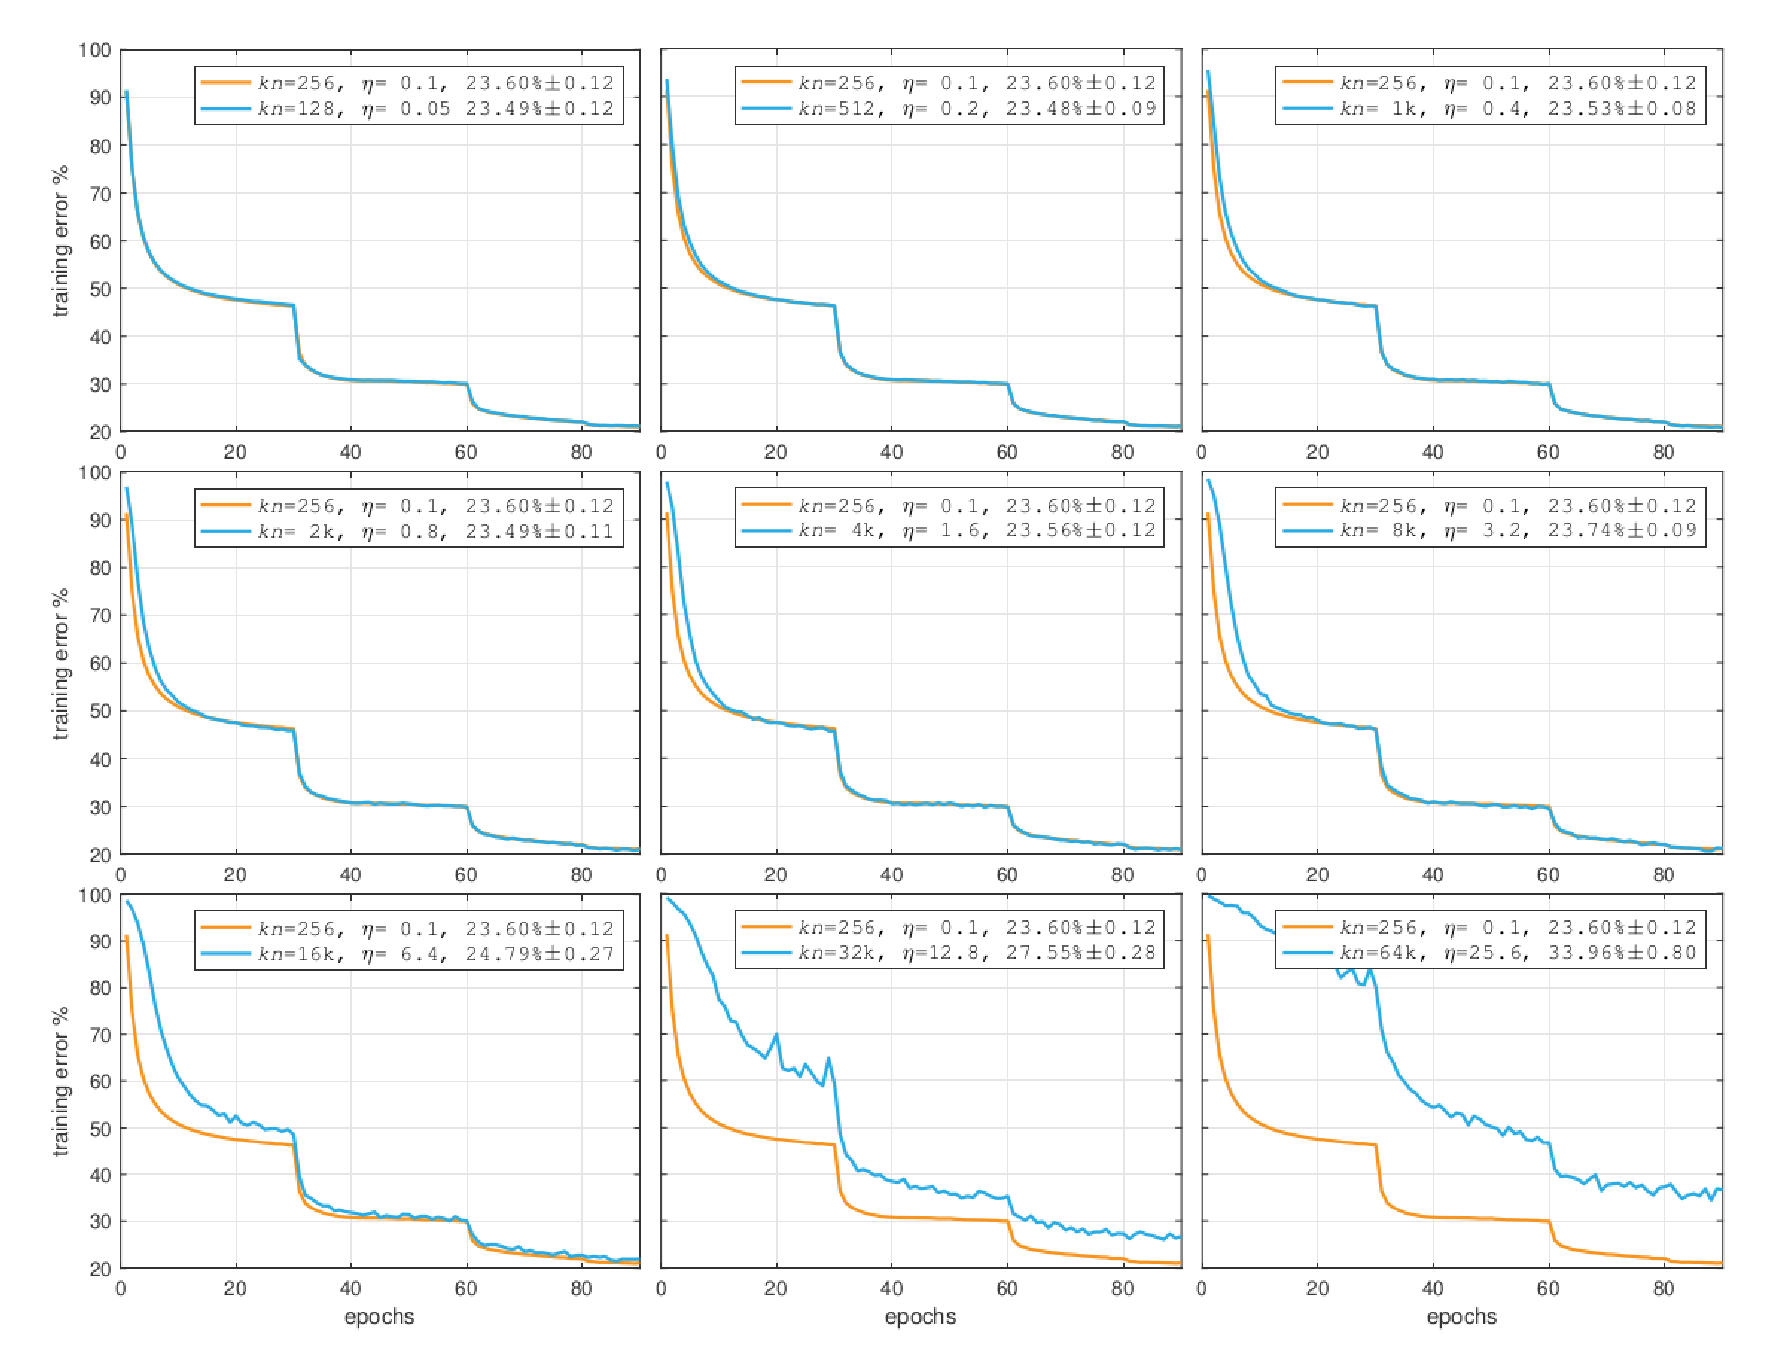
\includegraphics[width=0.85\textwidth,height=\textheight]{../files/sem_19_large_batch_results.pdf}
\end{column}

\begin{column}{0.2\textwidth}
The training curves closely match the baseline (aside from the warmup
period) up through \(8k\) minibatches.
\end{column}
\end{columns}
\end{frame}

\begin{frame}{Accurate, Large Minibatch SGD. Results on ImageNet}
\phantomsection\label{accurate-large-minibatch-sgd.-results-on-imagenet-1}
\begin{columns}[T]
\begin{column}{0.5\textwidth}
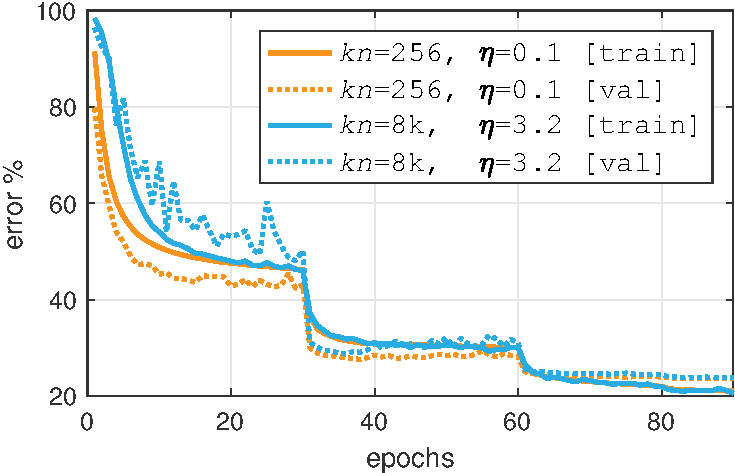
\includegraphics[width=1\textwidth,height=\textheight]{../files/sem_19_large_batch_train_val.pdf}
\end{column}

\begin{column}{0.5\textwidth}
Both sets of curves match closely after training for sufficient epochs.

Note that the BN statistics (for inference only) are computed using
running average, which is updated less frequently with a large minibatch
and thus is noisier in early training (this explains the larger
variation of the validation error in early epochs).
\end{column}
\end{columns}
\end{frame}

\section{Reduce memory usage}\label{reduce-memory-usage}

\begin{frame}{Reduce memory usage. CPU Offloading}
\phantomsection\label{reduce-memory-usage.-cpu-offloading}
\begin{itemize}
\item
  Offloading the weights to the CPU and only loading them on the GPU
  when performing the forward pass
\item
  CPU offloading works on submodules rather than whole models.
\item
  Inference is much slower due to the iterative uploading and
  offloading.
\item
  Colab Example
  \href{https://colab.research.google.com/drive/1Ugx3dUl_MHsYCAgz12qbuz_couJajpb6?usp=sharing}{\faPython Open
  in Colab}.
\end{itemize}
\end{frame}

\begin{frame}{Reduce memory usage. Model Offloading}
\phantomsection\label{reduce-memory-usage.-model-offloading}
\begin{itemize}
\item
  CPU Offloading makes inference slower because \emph{submodules} are
  moved to GPU as needed, and they're immediately returned to the CPU
  when a new module runs.
\item
  Full-model offloading is an alternative that moves whole models to the
  GPU, instead of handling each model's constituent \emph{submodules}.
\item
  During model offloading, only one of the main components of the
  pipeline (typically the text encoder, UNet or VAE) is placed on the
  GPU while the others wait on the CPU.
\item
  Colab Example
  \href{https://colab.research.google.com/drive/1Ugx3dUl_MHsYCAgz12qbuz_couJajpb6?usp=sharing}{\faPython Open
  in Colab}.
\end{itemize}
\end{frame}

\begin{frame}[fragile]{Reduce memory usage. Quantization}
\phantomsection\label{reduce-memory-usage.-quantization}
\begin{itemize}
\item
  Quantization maps a floating point value \(x \in [\alpha, \beta]\) to
  a \(b\)-bit integer \(x_q \in [\alpha_q, \beta_q]\).
\item
  The quantization process is defined as
  \[x_q = \text{clip}\Big( \text{round}\big(\frac{1}{s} x + z\big), \alpha_q, \beta_q \Big)\]
  And the de-quantization process is defined as \[x = s (x_q - z)\] The
  value of scale \(s\) and zero point \(z\) are \begin{align}
  s &= \frac{\beta - \alpha}{\beta_q - \alpha_q} \\
  z &= \text{round}\big(\frac{\beta \alpha_q - \alpha \beta_q}{\beta - \alpha}\big) \\
  \end{align} \textbf{Note} that \(z\) is an integer and \(s\) is a
  positive floating point number.
\item
  Quantization allows to perform a lot of heavy DL-operations
  (e.g.~matrix maltiplication) in integer scope using efficient integer
  hardware (\texttt{NVIDIA\ Tensor\ Core} or
  \texttt{Tensor\ Core\ IMMA\ operations}) and algorithms.
\end{itemize}
\end{frame}

\begin{frame}{Reduce memory usage. Quantization}
\phantomsection\label{reduce-memory-usage.-quantization-1}
\begin{itemize}
\item
  For more theory look at \emph{Quantization for Neural Networks }, Lei
  Mao:
  \href{https://leimao.github.io/article/Neural-Networks-Quantization/\#Quantization}{\faGit}.
\item
  Colab Example
  \href{https://colab.research.google.com/drive/1Ugx3dUl_MHsYCAgz12qbuz_couJajpb6?usp=sharing}{\faPython Open
  in Colab}.
\end{itemize}
\end{frame}

\begin{frame}{Mixed Precision Training (MPT)}
\phantomsection\label{mixed-precision-training-mpt}
\begin{center}
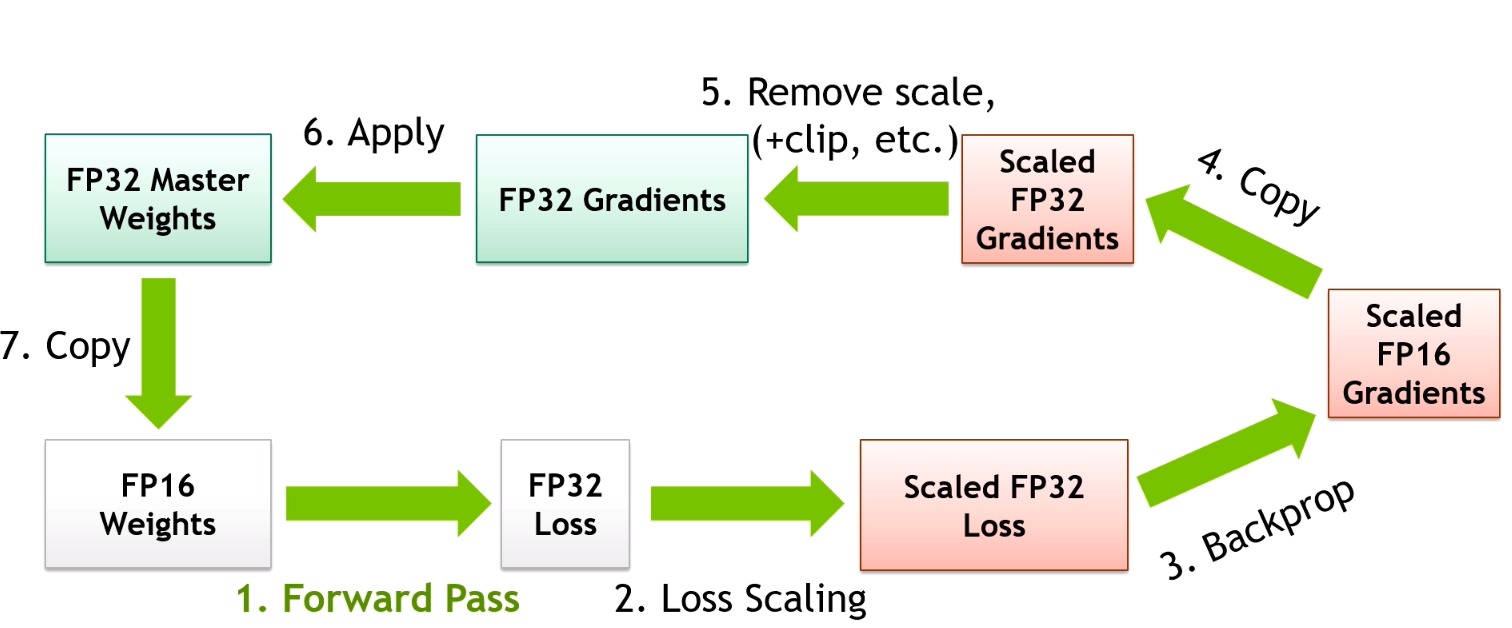
\includegraphics[width=0.75\textwidth,height=\textheight]{../files/MPT_vis.png}
\end{center}

Mixed Precision Training is a technique where both 16-bit (FP16) and
32-bit (FP32) floating-point types are used during neural network
training. This approach accelerates training and reduces memory usage
without compromising model accuracy.
\end{frame}

\begin{frame}{Why is MPT beneficial?}
\phantomsection\label{why-is-mpt-beneficial}
\begin{itemize}
\item
  \textbf{Faster Training}: Utilizing FP16 allows for faster
  computations, especially on modern GPUs equipped with Tensor Cores,
  such as NVIDIA Volta, Turing, and Ampere architectures. This can lead
  to training speedups of 2--3 times.
\item
  \textbf{Reduced Memory Consumption}: FP16 uses half the memory
  compared to FP32, enabling the training of larger models or the use of
  larger batch sizes.
\item
  \textbf{Maintained Accuracy}: With proper implementation, mixed
  precision training maintains the same level of model accuracy as full
  precision (FP32) training.
\end{itemize}
\end{frame}

\begin{frame}[fragile]{How does it work?}
\phantomsection\label{how-does-it-work}
\begin{enumerate}
\item
  \textbf{Autocasting}: Certain operations, like matrix multiplications
  and convolutions, are performed in FP16, while others that require
  higher precision remain in FP32. This is managed automatically in
  frameworks like PyTorch and TensorFlow.
\item
  \textbf{Loss Scaling}: To prevent small gradient values from
  underflowing in FP16, the loss is scaled up during backpropagation and
  then scaled down before the optimizer step.
\end{enumerate}

PyTorch \emph{example}:

\begin{Shaded}
\begin{Highlighting}[]
\ImportTok{from}\NormalTok{ torch.cuda.amp }\ImportTok{import}\NormalTok{ autocast, GradScaler}

\NormalTok{scaler }\OperatorTok{=}\NormalTok{ GradScaler()}

\ControlFlowTok{for}\NormalTok{ data, target }\KeywordTok{in}\NormalTok{ dataloader:}
\NormalTok{    optimizer.zero\_grad()}
    \ControlFlowTok{with}\NormalTok{ autocast():}
\NormalTok{        output }\OperatorTok{=}\NormalTok{ model(data)}
\NormalTok{        loss }\OperatorTok{=}\NormalTok{ loss\_fn(output, target)}
\NormalTok{    scaler.scale(loss).backward()}
\NormalTok{    scaler.step(optimizer)}
\NormalTok{    scaler.update()}
\end{Highlighting}
\end{Shaded}
\end{frame}

\begin{frame}{When to use Mixed Precision Training?}
\phantomsection\label{when-to-use-mixed-precision-training}
\begin{itemize}
\item
  Training on Modern GPUs: Particularly effective on GPUs with Tensor
  Cores (e.g., NVIDIA V100, A100).
\item
  Resource-Constrained Environments: Reduces memory consumption and
  accelerates training, beneficial when computational resources are
  limited.
\item
  See also an interesting blog post on the topic of Mixed Precision
  Training
  \href{https://blog.paperspace.com/mixed-precision-training-benchmark/}{\faFilePdf}
\end{itemize}
\end{frame}



\end{document}
